\chapter[Electron Charge Asymmetry]{Measurement of the Electron Charge Asymmetry
 with \unit{36}{\invpb} }

In this chapter the results of the measurement of the electron charge
asymmetry are presented. The analysis is performed on the full 2010 dataset, which corresponds to a
luminosity of \unit{36.1}{\invpb}.

The results are presented in 6 bins of absolute value of pseudorapidity with a
fixed width of 0.4. To avoid the gap between the ECAL barrel and ECAL endcap the
region $1.4<|\eta|<1.6$ is excluded.

\section{Event Selection}

The event selection is performed on single electron datasets formed of events
that are selected using various single photon and single electron triggers. From
these datasets, electrons are selected that pass a limited number of cuts.
Events that contain only a single electron are then selected for the analysis.

\subsection{Trigger}

Several triggers were used to select the events due to the increasing luminosity
during the \ac{LHC} 2010 run.  In the initial runs, events were selected using
only a single photon trigger.  As the \ac{LHC} luminosity was increased and
these triggers became prescaled, it was necessary to use electron triggers to
select events.  As the luminosity increased even further, it was necessary to use
electron triggers that included cuts on certain electron ID variables.

In the following analysis, a control region is obtained by inverting the
selection on the $\Delta\phi$ and $\Delta\eta$ variables. To ensure that this
inverted selection is effective and will actually select events, it is necessary
to avoid using triggers that apply a selection on these variables.

The triggers used to select the events are summarised in \TableRef{tab:triggers}
where ``HLT\_Ele$X$'' indicates a selection requiring an electron with  $\Pt > \unit{X}{\GeV}$. 
``Photon'' in the name indicates that the selection was applied to ECAL
superclusters rather than a reconstructed electron. 
``SW'' stands for small window, where window refers to the electron
pixel-matching window. 
 ``Cleaned'' indicates that spikes in the \ac{ECAL} have been removed.  

``CaloEleId'' and ``TightCaloIdIso'' represent increasingly tighter selection
based on the shower shape ID and isolation variables from only the \ac{ECAL},
and not the $\Delta\phi$ or $\Delta\eta$ variables.  

``TightCaloIdIso'' indicates a tight selection based on all ID variables. 
This nullifies the inverted cuts used for the control region but
it was the only trigger available for these runs without a prescale applied.
To compensate for the missing events in the control region, a looser prescaled
trigger was also applied in these runs.

\begin{table}[htbp]
  \centering
  \begin{tabular}{ l l }
    \toprule
    Run Ranges & Trigger String\\
    \midrule
    132440-137028 & \verb=HLT_Photon10_L1R= \\
    138564-140401 & \verb=HLT_Photon15_Cleaned_L1R= \\
    141956-144114 & \verb=HLT_Ele15_SW_CaloEleId_L1R= \\
    146428-147116 & \verb=HLT_Ele17_SW_CaloEleId_L1R= \\
    147196-148102 & \verb=HLT_Ele17_SW_TightEleId_L1R= \\
                  & \verb=HLT_Ele17_SW_L1R (prescaled)= \\ 
    148822-149063 & \verb=HLT_Ele22_SW_TighterCaloIdIso1_L1R_v1= \\
    149181-149442 & \verb=HLT_Ele22_SW_TighterCaloIdIso1_L1R_v2= \\
    \bottomrule
  \end{tabular}
  \caption{Triggers used to select the data used in this analysis.}
  \label{tab:triggers}
\end{table}

\subsection{Electron Selection}
The available triggers place a limit the electron \pT threshold to be
greater than \unit{25}{\GeV} in the analysis. 
The results are presented with an electron \pT cut of 25, 30
and \unit{35}{\GeV}.

Electron candidates are identified using a cut based approach on an limited
number of variables. The cut values used correspond to the \unit{80}{\%}
working point from \TableRef{tab:electronwp}, and are summarised again in
\TableRef{tab:electronselection}. The \unit{80}{\%} working point was chosen as a
compromise between ensuring suitable statistics while maintaining the purity of
the sample.

\begin{table}[htbp]
  \begin{center}
    \leavevmode
    \begin{tabular}{lll} 
    \toprule
      Selection Variable & \multicolumn{2}{c}{Cut Value}\\
                         & Barrel & Endcap\\
      \midrule
      \multicolumn{3}{l}{\emph{ID Cuts}}\\ 
        H/E & 0.04 & 0.025 \\
        $\Delta\phi$ & 0.06 & 0.03 \\
        $\Delta\eta$ & 0.004 & 0.007  \\
        $\sigma_{\eta\eta}$ & 0.01 & 0.03 \\ \midrule
      \multicolumn{3}{l}{\emph{Isolation Cuts}}\\
        $ISO_{trk} / E_T $  & 0.09 & 0.04 \\
        $ISO_{ecal}/ E_T$  & 0.07 & 0.05 \\
        $ISO_{hcal}/ E_T$  & 0.10 & 0.025 \\ \midrule
      \multicolumn{3}{l}{\emph{Conversion Rejection Cuts}}\\ 
        Missing Hits  & \multicolumn{2}{c}{$\leq 0$}\\
        Dist $||$ Dcot   & \multicolumn{2}{c}{$>0.02$}\\
    \bottomrule
    \end{tabular}
    \caption{\label{tab:electronselection} Electron selection variables and corresponding cut values.}
  \end{center}
\end{table}

Incorrectly assigning the charge of an electron will lead to a dilution of the
measured charge asymmetry.  An additional requirement is applied to the charge
of the reconstructed electron to reject events where the true charge is
difficult to determine.  The methods for assigning a charge to an electron are
described in \SectionRef{sec:charge}. The methods are based on the GSF electron
charge, the general track charge and the supercluster charge.
Electron candidates are only selected if the three methods unanimously agree on
its charge.

The incorrect charge assignment rate can be measured at the Z peak by comparing the same
sign \HepProcess{\PZ\to\Pepm\Pepm} yield to the opposite sign
\HepProcess{\PZ\to\Pepm\Pemp} yield. \FigureRef{fig:zpeak} show these Z yields
using only the \ac{GSF} track charge (red) and also requiring a unanimous
assignment of charge from all three methods (blue). 

The incorrect charge assignment rate from the GSF track charge alone is about
\unit{3}{\%}.  By requiring that all three methods for assigning the charge
agree, and vetoing events otherwise, the incorrect assignment rate can be
reduced by a factor of 8 with only a \unit{5}{\%} loss in efficiency.

\begin{figure}[htbp]
  \centering
  \begin{subfigure}{\textwidth}
    \centering
    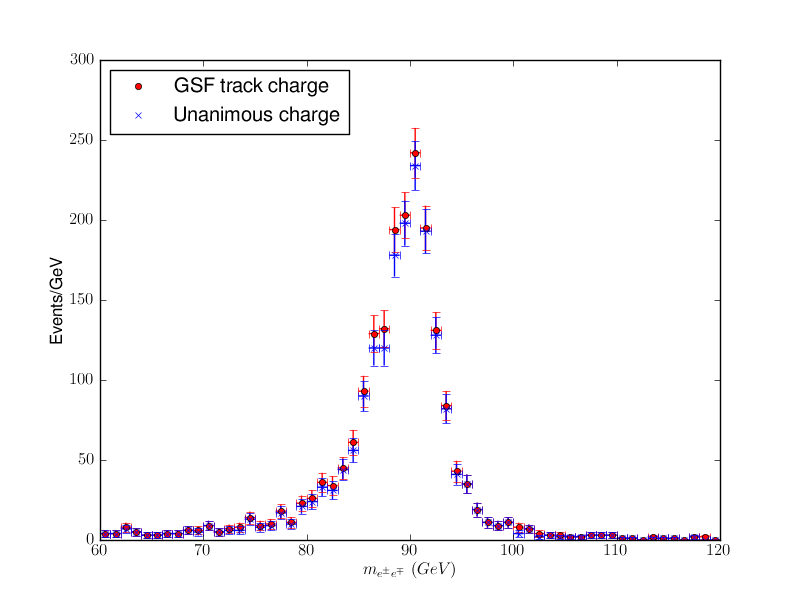
\includegraphics[width=0.85\textwidth]{zpeak_os}
    \caption{Opposite sign \PZ.}
    \label{fig:zpeak_os}
  \end{subfigure}
  \begin{subfigure}{\textwidth}
    \centering
    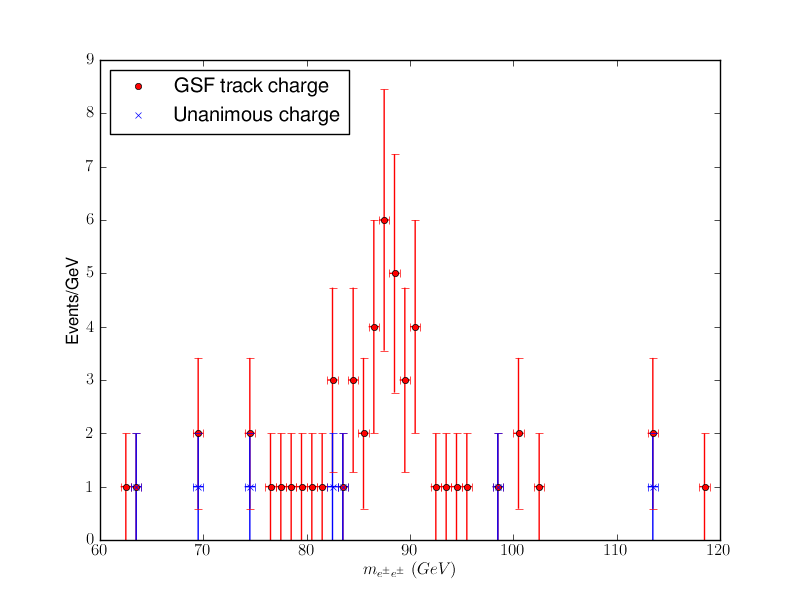
\includegraphics[width=0.85\textwidth]{zpeak_ss}
    \caption{Same sign \PZ.}
    \label{fig:zpeak_ss}
  \end{subfigure}
  \caption{ $Z\rightarrow ee$ peak. One electron is required to be in the
barrel to pass the VBTF80 selection and to have a fraction of energy loss by
radiation less than 0.3; the second electron is required only to pass the VBTF80
selection.}\label{fig:zpeak} 
\end{figure}

\subsection{Event Selection}
An event is selected if it contains a single electron that passes all the
electron selection requirements.  To remove Drell-Yan events, an event is vetoed
if it contains a second lepton (an electron passing a loose select on, or an
isolated muon) with $\PT > \unit{15}{\GeV}$.

The expected composition of the selected events, derived from MC simulation
samples, is shown in \TableRef{tab:selectedcomp}. With a \pT cut of
\unit{25}{\GeV} it is expected that the selected events are \unit{$\approx
65$}{\%} signal events, and of the remaing \unit{35}{\%} background events, the
majority of them are \ac{QCD} background events with a small amount of \ac{EWK}
events. 

\begin{table}[htbp]
\begin{center}
\begin{tabular}{llrrr}
    \toprule
& & $\PT>25$ \GeV & $\PT>30$ \GeV & $\PT>35$ \GeV  \\
\midrule
Signal & \HepProcess{\PW\to\Pe\Pnu} & $65.1\%$&$63.5\%$ &$60.2\%$ \\
EWK & \HepProcess{\PZ\to\Ptau\Ptau} & $0.4\%$ &$0.3\%$  &$0.2\%$ \\
    & \HepProcess{\PZ\to\Pe\Pe}     & $4.1\%$ &$3.5\%$  &$3.0\%$\\
    & \HepProcess{\PW\to\Ptau\Pnu}  & $1.9\%$ &$1.1\%$  &$0.6\%$\\
    & \HepProcess{\Ptop\APtop}      & $0.3\%$ &$0.3\%$  &$0.3\%$\\
    & Total                         & $6.7\%$ &$5.2\%$  &$4.1\%$\\
QCD & Total                         & $28.2\%$&$31.3\%$ &$35.7\%$\\
    \bottomrule
\end{tabular}
\caption{Composition of selected events for lepton momentum cut of $\PT>25$ \GeV, $\PT>30$ \GeV and $\PT>35$ \GeV .}
\label{tab:selectedcomp}
\end{center}
\end{table}

The Particle Flow \ETm distribution for the events that pass the event
selection, with an electron cut of $\PT > \unit{25}{\GeV}$ and $|\eta| < 2.4$ is
shown in \FigureRef{fig:pfmet}. There are two obvious peaks in the
distribution. The peak at \unit{$\ETm \approx 40$}{\GeV} is the
\HepProcess{\PW\to\Pelectron\Pnue} signal region. This region will also contain
\HepProcess{\PW\to\Ptau\Pnut} backgrounds. The peak at
\unit{$\ETm\approx 10$}{\GeV} is the background region that contains the \ac{QCD}
and \ac{DY} background events.

\begin{figure}[htbp]
  \begin{center}
    \includegraphics*[width=0.85\textwidth]{pfmet_dist}
    \caption{Particle Flow transverse missing energy (PFMET) distribution for selected events.}
  \label{fig:pfmet}
  \end{center}
\end{figure}

The number of selected events that pass the
event selection are shown in \TableRef{tab:selectedevents}. To obtain a
measurement of the asymmetry from the selected events it is necessary to extract
the signal yield from each pseudorapidity/charge bin.

\begin{table}[htbp]
\begin{center}
%\begin{sideways}
\begin{tabular}{lcrrr}
    \toprule
  $|\eta|$ range & Charge & \multicolumn{3}{c}{Selected Events}\\
                 &        & $\PT>25$ \GeV & $\PT>30$ \GeV & $\PT>35$ \GeV\\
\midrule
$0.0<| \eta |<0.4$ &+& 18956&14232&9885\\
                   &-& 15060&11505&8105\\
$0.4<| \eta |<0.8$ &+& 20118&14966&10345\\
                   &-& 15736&11780&8307\\
$0.8<| \eta |<1.2$ &+& 20681&15091&10184\\
                   &-& 16167&11735&8112\\
$1.2<| \eta |<1.4$ &+& 10646&7606&5161\\
                   &-& 8226&5871&4067\\
$1.6<| \eta |<2.0$ &+& 16426&11877&7814\\
                   &-& 11678&8578&5886\\
$2.0<| \eta |<2.4$ &+& 18885&13239&8726\\
                   &-& 13226&9227&6184\\
    \bottomrule
\end{tabular}
%\end{sideways}
\end{center}
\caption{Number of events passing the event selection for lepton momentum cut of $\PT>25$ \GeV, $\PT>30$ \GeV and $\PT>35$ \GeV .}
    \label{tab:selectedevents}
\end{table}


\section{Signal Yield Extraction Method}
The number of signal and background events in each bin is extracted using a fit
to the \ETm distribution using two templates.
The first is the sum of the \Wenu signal and the \ac{EWK} background shapes,
and the second is the sum of the \ac{QCD} plus \gjet processes.

\subsection{\ac{QCD} \ETm Shape}
The \ac{QCD} and \gjet background distribution is obtained from a control sample of
events. The control sample is selected by requiring that the electrons pass the
isolation and H over E cuts but fail the $\Delta\phi$ and $\Delta\eta$ cuts as
shown in \TableRef{tab:antisel}.

\begin{figure}[htbp]
  \centering
  \begin{subfigure}{0.45\textwidth}
    \centering
    \includegraphics*[trim = 0mm 0mm 15mm 0mm, clip, width=\textwidth, angle=90]{MetCompare_anti_eta1.pdf}
    \caption{test.}
    \label{fig:qcd_met_eta1}
  \end{subfigure}
  \begin{subfigure}{0.45\textwidth}
    \centering
    \includegraphics*[trim = 0mm 0mm 15mm 0mm, clip, width=\textwidth, angle=90]{MetCompare_anti_eta2.pdf}
    \caption{test.}
    \label{fig:qcd_met_eta2}
  \end{subfigure}
  \begin{subfigure}{0.45\textwidth}
    \centering
    \includegraphics*[trim = 0mm 0mm 15mm 0mm, clip, width=\textwidth, angle=90]{MetCompare_anti_eta3.pdf}
    \caption{test.}
    \label{fig:qcd_met_eta3}
  \end{subfigure}
  \begin{subfigure}{0.45\textwidth}
    \centering
    \includegraphics*[trim = 0mm 0mm 15mm 0mm, clip, width=\textwidth, angle=90]{MetCompare_anti_eta4.pdf}
    \caption{test.}
    \label{fig:qcd_met_eta4}
  \end{subfigure}
  \begin{subfigure}{0.45\textwidth}
    \centering
    \includegraphics*[trim = 0mm 0mm 15mm 0mm, clip, width=\textwidth, angle=90]{MetCompare_anti_eta5.pdf}
    \caption{test.}
    \label{fig:qcd_met_eta5}
  \end{subfigure}
  \begin{subfigure}{0.45\textwidth}
    \centering
    \includegraphics*[trim = 0mm 0mm 15mm 0mm, clip, width=\textwidth, angle=90]{MetCompare_anti_eta6.pdf}
    \caption{test.}
    \label{fig:qcd_met_eta6}
  \end{subfigure}
  \caption{The \ETm distribution on antiselected \ac{MC} simulated events and selected \ac{QCD} and \gjet events in each pseudorapidity bin.}
  \label{tab:antiselclosure}
\end{figure}

\begin{table}[htbp]
  \begin{center}
    \leavevmode
    \begin{tabular}{lcc} 
    \toprule
      Selection Variable & \multicolumn{2}{c}{Cut Value}\\
                         & Barrel & Endcap\\
    \midrule
        H/E & 0.04 & 0.025 \\
        $\Delta\phi$ & $>0.06$  & $>0.04$ \\
        $\Delta\eta$ & $>0.007$ & $>0.009$\\
        $ISO_{trk} / E_T $ & 0.09 & 0.04 \\
        $ISO_{ecal}/ E_T$  & 0.07 & 0.05 \\
        $ISO_{hcal}/ E_T$  & 0.10 & 0.025\\ 
    \bottomrule
    \end{tabular}
    \caption{\label{tab:antisel}Electron anti-selection variables and corresponding cut values. $\Delta\phi$ and $\Delta\eta$ cuts are inverted.}
  \end{center}
\end{table}

To validate the antiselection used, \ac{QCD} \ac{MC} samples are used. The
distribution of \ac{QCD} events passing the event selection are compared to the
antiselected MC events. This is shown for each eta bin in
\FigureRef{tab:antiselclosure}.

\subsection{Signal \ETm Shape from Boson Recoil}
\label{sec:recoil}
The signal \ETm shape is obtained by modelling the recoil of the W boson. 
The recoil response and resolution in \HepProcess{\PZ\to\Plepton\Plepton} data
events is measured as a function of the \pT of the boson. This is combined with
information from the \PW and \PZ \ac{MC} simulation to derive a correction to
the simulation \ETm as a function of \PW \pT.

The transverse recoil vector, $\vec{U}$, is calculated from the reconstructed
transverse missing energy, $\vec{\ETm}$, and the electron \ET vectors,
$\vec{\Pe_{i}}$.
\begin{align}
\vec{U} &= - \vec{\ETm} - \vec{\Pe},\\
\vec{U} &= - \vec{\ETm} - \sum_i \vec{\Pe_{i}},
\end{align}
for \PW events and \PZ events respectively. $\vec{U}$ is split into components
that are parallel ($U_1$) and perpendicular ($U_2$) to the true boson \pT
direction. 
In real \PZ data events where the true direction of the boson \pT is not known,
the \pT direction is reconstructed from the two electrons.
The hadronic activity that balances the \pT of boson will lie mostly in the
$U_1$ direction where as $U_2$ will be mostly formed from other sources.
\FigureRef{fig:recoil} shows the decomposition of $\vec{U}$ in to $U_1$ and
$U_2$ in W events.
\begin{figure}
  \begin{center}
    \includegraphics*[width=0.85\textwidth]{recoildiag}
    \caption{The decomposition of $\vec{U}$ for \PW events. From \cite{recoil}.}
    \label{fig:recoil}
  \end{center}
\end{figure}

$U_1$ and $U_2$ are measured in \PZ data, \PZ \ac{MC} simulation and \PW \ac{MC}
simulation and are then binned in units of the boson \pT.  In each $p_T^{Z}$ bin
the $U_1$ and $U_2$ distributions are fitted with Gaussian.  A polynomial,
$f_i(p_T^Z)$, is fit to the distribution of Gaussian the means to produce a
response curve for both data and \ac{MC}.  A second polynomial,
$\sigma_i(p_T^Z)$, is then fit to the distribution of the Gaussian widths to
produce a resolution curve for both data and \ac{MC}.

The fitting procedure results in two response functions, $f_i(p_T^Z)$, and two
resolution function, $\sigma_i(p_T^Z)$, for \PZ data, \PZ \ac{MC} and the \PW
\ac{MC}. The functions are then used to define a set of \PW \ac{MC} corrected
functions, 

\begin{align}
f^{corr}_i (p^{W}_T)      
  &= \frac{ f^{Z\ data}_i (p^{Z}_T) }
          { f^{Z\ MC}_i (p^{Z}_T) }
          f^{W\ MC}_i (p^{W}_T) \\
\sigma^{corr}_i (p^{W}_T) 
  &= \frac{ \sigma^{Z\ data}_i (p^{Z}_T) }
          { \sigma^{Z\ MC}_i (p^{Z}_T) }
          \sigma^{W\ MC}_i (p^{W}_T) 
\end{align}

The corrected recoil response and resolution curves are then used to correct the
\PW \ac{MC} \ETm. For each \PW \ac{MC} events the real \pT of the boson is
found, and the values of for the response, $f^{corr}_i (p^{W}_T)$, and
resolution curves, $\sigma^{corr}_i (p^{W}_T) $, are looked up. A Gaussian is
defined with these values and then sampled to determine the new recoil
components $U_i$.
\begin{equation}
U_i \sim Gaus(f^{corr}_i (p^{W}_T), \sigma^{corr}_i (p^{W}_T) )
\end{equation}
The components are then combined to form the new corrected recoil vector
$\vec{U^{\prime}}$ which is then combined with the electron vector, $\Pe$, to
form the corrected \ETm.

The modelling of the \HepProcess{\PW\to\Plepton\Pnu} \ETm with boson recoil is
described in detail here \cite{NULL}, and the ntuples containing
\HepProcess{\PW\to\Pelectron\Pnu} simulation with the recoil corrected \ETm were
provided from here \cite{NULL}.

\subsection{\ac{EWK} \ETm Shape}
The EWK background processes that can produce a single isolated
electron which are considered in this analysis are:
\begin{itemize}
\item \HepProcess{\PZ\to\Pelectron\APelectron},
\item \HepProcess{\PZ\to\Ptauon\APtauon},
\item \HepProcess{\PW\to\Ptau\Pnu},
\item \HepProcess{\Ptop\APtop}.
\end{itemize}

The \ac{EWK} background \ETm distributions were obtained from Pythia \ac{MC}
simulations for each pseudorapidity/charge bin.  The scale of the \ac{EWK} shape
is fixed to the signal \ETm shape by the ratio obtained from \ac{MC} samples.

\subsection{Validation of Signal Extraction Method on Simulation}

The signal yield extraction procedure was validated using pseudo-data
experiments. 1000 pseudo-data experiments were generated with the number of
events expected in \unit{36.1}{\invpb} of data. The signal yields are extracted
in each experiment and the asymmetry is calculated. The distribution of
asymmetries is then fitted with a Gaussian.
The measured asymmetry for 1000 pseudo-data experiments distribution for each
pseudorapidity bin is shown in \FigureRef{fig:toyasym}.

The width of the Gaussian is the statistical uncertainty on the measurement.
The statistical uncertainty can also be estimated from the following formula
\begin{equation}
  \label{tab:statuncert}
   \frac{d\mathcal{A}_{stat}}{d\eta} =
   \frac{2 \times \sqrt{ 
       \left( \frac{dN^+}{d\eta} \sigma_{\frac{dN^-} {d\eta}}\right)^2 + 
       \left( \frac{dN^-}{d\eta} \sigma_{\frac{dN^+} {d\eta}}\right)^2  }}
   {\left(  \frac{dN^+}{d\eta} +  \frac{dN^-}{d\eta} \right)^{2} } .
\end{equation}

The uncertainty from \EquationRef{tab:statuncert} evaluated with \ac{MC} truth
values, and the uncertainty measured from pseudo-data experiments for an
integrated luminosity of \unit{36.1}{\invpb} are summarised in
\TableRef{tab:statuncertsum}.

\begin{table}[htbp]
  \begin{center}
    \begin{tabular}{lcc}
    \toprule
    $|\eta|$ range & $\sigma_{A}$ from \EquationRef{tab:statuncert}. & $\sigma_{A}$ from pseudo-data exp.\\ \midrule
    $0.0<|\eta|<0.4$ & 0.0064 & 0.0062\\
    $0.4<|\eta|<0.8$ & 0.0064 & 0.0064\\
    $0.8<|\eta|<1.2$ & 0.0065 & 0.0065\\
    $1.2<|\eta|<1.4$ & 0.0096 & 0.0104\\
    $1.6<|\eta|<2.0$ & 0.0076 & 0.0079\\
    $2.0<|\eta|<2.4$ & 0.0077 & 0.0077\\
    \bottomrule
    \end{tabular}
  \caption{Expected statistical error as a function of pseudorapidity, for an
  integrated luminosity of \unit{36}{\invpb}. }
  \label{tab:statuncertsum}
  \end{center}
\end{table}

For each pseudo-data experiment the pull on the asymmetry measurement is
calculated. The pull is defined as the difference between the asymmetry measured
from pseudo-data experiments and the true MC value for the asymmetry divided by
the statistical uncertainty. The pull is therefore the number of standard
deviations a measurement is away from the true value such that, for an unbiased
measurement with a well understood uncertainty, the distribution of the pulls
will be a Gaussian centred at zero with a width of one.
The pull distributions from 1000 pseudo-data experiments are shown in figure
\ref{fig:toyasym_pull} for each pseudorapidity bin.

\begin{figure}[htbp]
  \begin{center}
    \includegraphics*[angle=90,width=0.95\textwidth]{toyasym.pdf}
    \caption{\label{fig:toyasym}Measured Asymmetry for 1000 pseudo-data experiments. The distribution of the measured Asymmetry is fitted with a Gaussian.}
  \end{center}
\end{figure}

\begin{figure}[htbp]
  \begin{center}
\includegraphics*[angle=90,width=0.95\textwidth]{pullasyTot.pdf}
    \caption{\label{fig:toyasym_pull}Pull on the Asymmetry in 1000 pseudo-data experiments. The distribution of the pull is fitted with a Gaussian.}
  \end{center}
\end{figure}

\subsection{Fit Results}

The results of the extended maximum likelihood fits to each pseudorapidity/charge
bin are shown in \FigureRef{fig:fit1} and \FigureRef{fig:fit2}.
The ratio between the fits and the data for each of the 
bins are shown in \FigureRef{fig:fit1ratio} and \FigureRef{fig:fit2ratio}.
The signal yield in each bin is summarised in \TableRef{tab:sigyield} and the
$\chi^2$ of each fit is noted in \TableRef{tab:chi2}.

\begin{table}[htbp]
\begin{center}
%\begin{sideways}
\begin{tabular}{lcrrr}
    \toprule
$|\eta|$ range & Charge & \multicolumn{3}{c}{Signal Yield}\\
               &        & $\PT>25$ \GeV & $\PT>30$ \GeV & $\PT>35$ \GeV  \\
\midrule
$0.0<| \eta |<0.4$ &+&-&-&-\\
                   &-&-&-&-\\
$0.4<| \eta |<0.8$ &+&-&-&-\\
                   &-&-&-&-\\
$0.8<| \eta |<1.2$ &+&-&-&-\\
                   &-&-&-&-\\
$1.2<| \eta |<1.4$ &+&-&-&-\\
                   &-&-&-&-\\
$1.6<| \eta |<2.0$ &+&-&-&-\\
                   &-&-&-&-\\
$2.0<| \eta |<2.4$ &+&-&-&-\\
                   &-&-&-&-\\
    \bottomrule
\end{tabular}
%\end{sideways}
\end{center}
\caption{Signal yield}
    \label{tab:sigyield}
\end{table}

\begin{table}[htbp]
\begin{center}
\begin{tabular}{lcr}
    \toprule
$|\eta|$ range &Charge & $\chi^2$/ndof of Fit\\
\midrule
$0.0<| \eta |<0.4$ &+&  0.86\\
                   &-&  0.84\\
$0.4<| \eta |<0.8$ &+&  0.99\\
                   &-&  1.36\\
$0.8<| \eta |<1.2$ &+&  1.05\\
                   &-&  1.13\\
$1.2<| \eta |<1.4$ &+&  0.97\\
                   &-&  1.30\\
$1.6<| \eta |<2.0$ &+&  1.38\\
                   &-&  1.61\\
$2.0<| \eta |<2.4$ &+&  1.44\\
                   &-&  1.11\\
    \bottomrule
\end{tabular}
\caption{\label{tab:chi2}$\chi^2$/ndof of Fit.}
\end{center}
\end{table}


\section{Corrections to the Measured Asymmetry}
After the signal extraction procedure the measured asymmetry is simply 
\begin{equation}
\mathcal{A}_{meas} = \frac{
\label{eq:meas}
  N_{meas}^{+} -
  N_{meas}^{-}
}
{
  N_{meas}^{+} +
  N_{meas}^{-}
}
\end{equation}
where $N_{meas}^{+}$ and $N_{meas}^{-}$ are number of positrons and
electrons extracted with the fitting procedure.
To compare with the theoretical value, the measured lepton asymmetry has to be
corrected for three detector effects.
\begin{itemize}
\item The charge-dependent Reconstruction efficiency,
\item The incorrect charge assignment rate,
\item Electron energy resolution.
\end{itemize}

If the reconstruction efficiency of electrons ($\epsilon^-$) is different to
that of positrons ($\epsilon^-$) then a bias will be introduced in to the
measured asymmetry, which will need to be taken in to account in the calculation
of the asymmetry.  

The second experimental effect is due the charge miss-assignment of electrons.
The incorrect charge assignment rates, $\omega^+$ and $\omega^-$ are the rate at which electrons are
incorrectly assigned a positive charge and identified as positrons and rate positrons are
identified as electrons respectively.
The incorrect assignment induces a dilution factor to the asymmetry as a
function of the electron pseudorapidity. 

The true asymmetry at the reconstruction level is defined as
\begin{equation}
\label{eq:reco}
\mathcal{A}_{reco} = \frac{
  N_{reco}^{+} -
  N_{reco}^{-}
}
{
  N_{reco}^{+} +
  N_{reco}^{-}
}
\end{equation}
where $N_{reco}^{+}$ and $N_{reco}^{-}$ are the true number of positrons and
electrons with \pT greater than the threshold. 
$N_{meas}^{+}$, $N_{meas}^{-}$ and 
$N_{reco}^{+}$, $N_{reco}^{-}$ are related by the efficiency of electrons and
positrons and the incorrect charge assignment rate.
\begin{align}
  \label{eq:poscor}
  N_{meas}^{+} 
  &= \epsilon^+ \left( ( 1 - \omega^- ) N_{reco}^{+} + \omega^+ N_{reco}^{-} \right)\\
  \label{eq:negcor}
  N_{meas}^{-} 
  &= \epsilon^+ \left( ( 1 - \omega^+ ) N_{reco}^{-} + \omega^- N_{reco}^{+} \right)
\end{align}


\EquationRef{eq:poscor} and \EquationRef{eq:negcor} can then be inserted in to the
definition of the measured asymmetry, \EquationRef{eq:meas}, to obtain,

\begin{equation}
\label{eq:meas1}
\mathcal{A}_{meas} = \frac{
  \epsilon^+ ( ( 1 - \omega^- ) N_{reco}^{+} + \omega^+ N_{reco}^{-} ) -
  \epsilon^+ ( ( 1 - \omega^+ ) N_{reco}^{-} + \omega^- N_{reco}^{+} )
}
{
  \epsilon^+ ( ( 1 - \omega^- ) N_{reco}^{+} + \omega^+ N_{reco}^{-} ) +
  \epsilon^+ ( ( 1 - \omega^+ ) N_{reco}^{-} + \omega^- N_{reco}^{+} )
}
\end{equation}
If it is assumed that the rate that
electrons are assigned a positive charge is the same as the rate of positrons
being assigned a negative charge, \ie 
\begin{equation}
  \omega^{+} = \omega^{-} = \omega
\end{equation}
then the dilution factor can be simplified to $(1-2\omega)$. A further
simplification is to introduce the relative detection efficiency, which is
defined as the ratio of electron efficiency to the positron efficiency,
\begin{equation}
 R = \epsilon^+/\epsilon^-
\end{equation}
which can be substituted in to \EquationRef{eq:meas1},
\begin{align}
\mathcal{A}_{meas} 
&= \frac{
  N_{reco}^{+} (R - \omega(R+1)) -
  N_{reco}^{-} (1 - \omega(R+1))
}
{
  N_{reco}^{+} (R - \omega(R-1)) +
  N_{reco}^{-} (1 + \omega(R-1))
}\\
&= \frac{
  (1+\mathcal{A}_{reco}) (R - \omega(R+1)) -
  (1-\mathcal{A}_{reco}) (1 - \omega(R+1))
}
{
  (1+\mathcal{A}_{reco}) (R - \omega(R+1)) -
  (1-\mathcal{A}_{reco}) (1 + \omega(R-1))
}\\
&= \frac{
  \mathcal{A}_{reco} (R + 1)(1 - 2 \omega) + (R - 1)
}
{
  \mathcal{A}_{reco} (R - 1)(1 - 2 \omega) + (R - 1)
}
\end{align}
which can then be inverted to derive $\mathcal{A}_{reco}$ as a function of the
measured asymmetry ($\mathcal{A}_{meas}$), the relative efficiency ($R$) and the
incorrect charge assignment rate ($\omega$).
\begin{align}
\mathcal{A}_{reco}
&=\frac{1}{1-2\omega}
  \frac{
    \mathcal{A}_{meas} (R + 1) - (R-1)
  }
  {
    (R + 1) - \mathcal{A}_{meas} (R-1)
  }\\
&\approx \frac{1}{1-2\omega}
\left(
  \mathcal{A}_{meas} -
\frac{ (R - 1)(1 - \mathcal{A}_{meas}^{2}) } { 2 }
\right)
\end{align}

The measurements of the parameters $R$ and $\omega$, as well as the
uncertainties, are detailed in the following sections.

The energy resolution and scale of the electrons can also introduce a systematic
bias on the asymmetry due to the effect of of the transverse momentum cut
applied to the electrons. The largest source of electron scale bias is the
radiation induced change to the ECAL crystal transparency.
To correct for this effect, energy scale and resolution corrections are
derived using a \Zee mass distribution. Te results are presented in the
following sections.

\subsection{Relative Efficiency}

If the reconstruction efficiency of electrons is different to that of positrons
then the measured asymmetry will be diluted and will need to be corrected for
the relative efficiency.

The efficiency for electrons and positrons is measured using the tag and probe
method \cite{tagandprobe}
with a sample of \Zee events from the same datasets used in the analysis. 
The \Zee events offer a high purity source of unbiased electrons with which to
measure the efficiencies.

From the sample of \Zee events a ``tag'' electron is selected with a strict
selection criteria. 
A ``probe'' electron is selected with the same electron selection described
earlier.
The invariant mass of the tag-probe pair is required to be
$\unit{60}{\GeV} < M_{ee} < \unit{120}{\GeV}$ to ensure a high purity sample.

Efficiencies can then be calculated by measuring the signal yield in events
with one tag electron and one probe passing the selection (tag \& pass) and
events where the probe electron fails the selection (tag \& fail).
The signal yield is extracted using an simultaneous maximum likelihood fit to
both the tag \& pass and the tag \& fail samples.

For this analysis the efficiencies are measured in two parts:

\begin{itemize}
    \item GSF tracking efficiency
    \item Identification efficiency, including conversion rejection, unanimous
charge assignment and HLT request.
\end{itemize}

\begin{table}[htbp]
\begin{center}
\begin{sideways}
\begin{tabular}{cccccccc}
    \toprule
$|\eta|$  & \multicolumn{3}{c}{GSF tracking } & \multicolumn{3}{c}{ID } & $R_\epsilon$ \\
region    & $\epsilon_{GSF}^+$ (\%) &$\epsilon_{GSF}^-$ (\%) & $R_{\epsilon_{GSF}}$ 
                                              & $\epsilon_{ID}^+$ (\%) &$\epsilon_{ID}^-$ (\%) & $R_{\epsilon_{ID}}$ &  \\
\midrule
$\left[ 0.0,0.4 \right]$ & 95.7$\pm$1.1 & 97.5$\pm$1.0 & 0.982$\pm$0.015 & 71.2$\pm$1.5 & 68.4$\pm$1.5 & 1.04$\pm$0.03 &1.02$\pm$0.035  \\
$\left[ 0.4,0.8 \right]$ & 98.8$\pm$ 1.0& 98.5$\pm$1.1 & 1.003$\pm$0.015 & 72.5$\pm$1.7 & 75.6$\pm$1.6 & 0.96$\pm$0.04 &0.96$\pm$ 0.04 \\
$\left[ 0.8,1.2 \right]$ & 97.6$\pm$ 1.0& 98.4$\pm$1.0 & 0.992$\pm$0.015 & 77.4$\pm$1.5 & 74.4$\pm$1.7 & 1.04$\pm$0.04 &1.03$\pm$ 0.04 \\
$\left[ 1.2,1.4 \right]$ & 96.2$\pm$ 1.5& 96.3$\pm$1.5 & 0.999$\pm$0.022 & 69.3$\pm$2.7 & 73.0$\pm$2.6 & 0.95$\pm$0.05 &0.95$\pm$0.05  \\
$\left[ 1.6,2.0 \right]$ & 96.8$\pm$ 1.2& 96.9$\pm$1.0 & 0.999$\pm$0.015 & 61.9$\pm$2.0 & 63.6$\pm$2.0 & 0.97$\pm$0.05 &0.97$\pm$0.05  \\
$\left[ 2.0,2.4 \right]$ & 96.4$\pm$ 1.1& 97.0$\pm$1.0 & 0.994$\pm$0.015 & 58.2$\pm$2.1 & 56.7$\pm$2.1 & 1.03$\pm$0.05 &1.02$\pm$0.05  \\
\midrule
$\left[ 0.0,1.4 \right]$ & 98.8$\pm$0.5 & 98.4 $\pm$0.5 & 1.004$\pm$0.007 & 84.1$\pm$0.8 & 83.8$\pm$0.8 & 1.003$\pm$0.014 & 1.007$\pm$ 0.015 \\
$\left[ 1.6,2.4 \right]$ & 98.3$\pm$0.7 & 97.8 $\pm$0.7 & 1.005$\pm$0.010 & 70.7$\pm$1.4 & 71.5$\pm$1.4 & 0.99$\pm$0.03 &0.99$\pm$ 0.03 \\
\midrule 
$\left[ 0.0,2.4 \right]$ & 98.5$\pm$0.4 & 97.8$\pm$0.4 & 1.007$\pm$0.006 & 80.3$\pm$0.7 & 80.3$\pm$0.7 & 1.000$\pm$0.012 &1.007$\pm$0.014  \\
    \bottomrule
\end{tabular}
\end{sideways}
\end{center}
\caption{ GSF tracking and identification efficiency as a function of charge.}
\label{tab:tagprobe}
\end{table}

The \TableRef{tab:tagprobe} shows the GSF tracking efficiency and identification 
efficiency as a function of the charge.


The main systematic errors on the efficiency measurements are the energy scale
and the signal shape used to extract the signal yield. Fortunately, these
errors will cancel in the calculation of the ratio $R_\epsilon$, such that the
effect of the energy scale and signal shape is negligible
when compared to the statistical uncertainty of the measurement. Only the
statistical uncertainty is therefore propagated to the error in the ratio
$dR_\epsilon$,
\begin{equation}
  \label{eq:releff}
  \sigma_{\mathcal{A}} 
  = \mathcal{A}(R_\epsilon=1) - \mathcal{A}(R_\epsilon=1\pm dR_\epsilon)  
  \simeq \frac{dR_\epsilon}{2}(1-\mathcal{A}^2)
  \simeq \frac{dR_\epsilon}{2} 
\end{equation}
The value of $R$ is measured in each pseudorapidity bin, as well as inclusively
across the range $0<| \eta |< 2.4$. 
The relative efficiency is found to be statistically compatible with 1 so the
measured asymmetry is not corrected for this effect.
In order to reduce the systematic error due to the effect of the relative
efficiency the statistical error on the inclusive measurement of $R$ is
propagated to the asymmetry as a systematic error. The systematic error assigned
in each bin is therefore $0.070$.

\subsection{Charge Misassignment}

The incorrect charge assignment rate, $\omega$, is the rate at which electrons are
wrongly assigned a positive charge and identified as positrons, and vice versa.
The effect of incorrectly assigning the charge is to dilute the measured
asymmetry.

The main mechanism responsible for the incorrect assignment of charge is the
conversion of bremsstrahlung photons close to the initial track, which the GSF
track reconstruction then incorrectly reconstructs.

The rate of incorrect charge assignment is obtained from \Zee samples selected from
real data  with the same selection used in the analysis. 
The rate is measured by comparing the
same sign \PZ\ yield (\HepProcess{\PZ\to\Pepm\Pepm}) to the opposite sign \PZ\
yield (\HepProcess{\PZ\to\Pepm\Pemp}).
It was found that the rate at which electrons are reconstructed as positrons is
the same as the rate of positrons reconstructed as electrons.
The total Z yield from this sample is 6834 opposite sign \PZ candidates and 21
same sign \PZ candidates.
The sample is split in to 21 sub-samples, representing
combinations of the 6 pseudorapidity bins of the two electrons ($6+\binom{6}{2} =
21$).

For each \PZ events with two electrons in pseudorapidity bin $i$ and $j$
respectively the probability of an event being same sign or opposite sign can be
written
\begin{equation}
%\[
 p(q_i q_j) =
  \begin{cases}
\left( 1-\omega_{i} \right) \left( 1-\omega_{j} \right) + \omega_{i} \omega_{j}
   & \text{if } q_1 q_2 =-1 \\
\omega_{i} \left( 1-\omega_{j} \right) + \omega_{j} \left( 1-\omega_{i} \right) 
   & \text{if } q_1 q_2 =+1 \\
  \end{cases}
%\]
\end{equation}
where $ \omega_{i},\omega_{j}$ are the incorrect charge assignment rates and $
q_{i},q_{j}$ are the charges of the electrons.

The incorrect charge assignment rates in each of the 6 pseudorapidity bins can then be
determined by a simultaneous fit to each of the 21 sub-samples. The results are
shown in \FigureRef{tab:mischarge}. The charge asymmetry is corrected for these
values.
The statistical error on the measurement on $\omega$ is then propagated to the
charge asymmetry as a systematic uncertainty, $\sigma(\mathcal{A})_{misch}$.

\begin{table}[htbp]
  \begin{center}
\begin{tabular}{lrrrr}
\toprule
$\eta$ range        & $\omega \times 10^{-4}$  & \multicolumn{3}{c}{$\sigma(\mathcal{A})_{misch}\times 10^{-4}$}\\
& & \PT $>$ 25 \GeV & \PT $>$ 30 \GeV & \PT $>$ 35 \GeV \\
\midrule
$0.0<| \eta |<0.4$  & $0^{+8}$          &  2 &  2 & 2 \\ 
$0.4<| \eta |<0.8$  & $8^{+8}_{-8}$     &  3 &  2 & 2 \\
$0.8<| \eta |<1.2$  & $11^{+10}_{-8}$   &  3 &  3 & 3 \\
$1.2<| \eta |<1.4$  & $34^{+21}_{-15}$  &  8 &  7 & 6 \\
$1.6<| \eta |<2.0$  & $41^{+20}_{-15}$  &  9 &  8 & 7 \\
$2.0<| \eta |<2.4$  & $25^{+21}_{-15}$  & 10 & 10 & 9 \\
\bottomrule
\end{tabular}
\caption{\label{tab:mischarge}Incorrect charge assignment rate and systematic effect on the charge asymmetry.}
\end{center}
\end{table}

\subsection{Lepton Energy Scale and Resolution}

The energy resolution and scale of the electrons can introduce a systematic
error on the asymmetry due to the effect of of the transverse momentum cut
applied to the electrons. The largest source of electron scale bias is the
changing ECAL crystal transparency caused by the changing level of radiation
during the \ac{LHC} 2010 run.

To correct for this effect, a set of ad-hoc energy scale and resolution corrections are
derived using a \Zee mass distribution. The corrections are parametrised by
six energy scale factors, $s_i$, and six resolutions, $\sigma_i$, one for each
pseudorapidity bin in the asymmetry measurement.
The scale factors represent the average factor each \ac{MC} electron's \Pt
should be corrected to match what is observed in data.
The resolution factors represent the difference of the resolution in data and
\ac{MC}. It is the additional smearing that would need to be applied to
reconstruction level \ac{MC} to match the observed resolution in data.

A sample of \Zee events is  split in to 21 categories which correspond to all
combinations of pseudorapidity bins of the two electrons ($6+\binom{6}{2} =
21$).  A mass template s obtained in each category from \ac{MC} simulation where
the \ac{ECAL} calibration is taken to be perfect.
A simultaneous fit to the \Zee mass is performed in each of the 21 categories
to determine the six energy scale factors, $s_i$, and the six resolutions, 
$\sigma_i$.

In each category ($category_{ij}$) where one electron is in the $i^{th}$
pseudorapidity bin and the other is in the $j^{th}$ bin, the \ac{MC} template
mass shape is scaled by $\frac{1}{\sqrt{s_i s_j} } $
and smeared by an additional Gaussian with width of
$\sqrt{\sigma_i^2+\sigma_j^2}$.

The corrections are applied to the electron before the final \Pt cut so that
the measured asymmetry is corrected for the energy scale.

A conservative uncertainty of \unit{1}{\% } is assigned to the electron energy
after the scale corrections. A systematic error is then estimated by measuring
the difference of the measured charge asymmetry with and without the additional
\unit{1}{\% } scale factor.

\begin{table}[htbp]
  \begin{center}
    \begin{tabular}{cccc}
    \toprule
$\eta$ range& $\sigma{\mathcal{A}} \times 10^{-4}$  & Additional $\sigma{E_{e^\pm}}$  & $\sigma{\mathcal{A}} \times 10^{-4}$ \\
& Perfect ECAL  & from fit  &  Realistic ECAL\\
& Calibration & (GeV) & Calibration \\
\midrule
$0.0<| \eta |<0.4$  &  8  & 0.2  &  4 \\
$0.4<| \eta |<0.8$  &  7  & 0.4  &  5\\
$0.8<| \eta |<1.2$  & 17  & 0.3  & 19\\
$1.2<| \eta |<1.4$  & 41  & 1.0  & 43\\
$1.6<| \eta |<2.0$  & 31  & 0.9  & 32 \\
$2.0<| \eta |<2.4$  & 41  & 0.3  & 42\\
    \bottomrule
    \end{tabular}
    \caption{\label{tab:acc}Systematic error for detector effects in the acceptance corrections.}
  \end{center}
\end{table}

\begin{table}[htbp]
  \begin{center}
    \begin{tabular}{cccc}
    \toprule
$\eta$ range& \PT $>$ 25 \GeV & \PT $>$ 30 \GeV & \PT $>$ 35 \GeV \\
\midrule
$0.0<| \eta |<0.4$  & 4 & 5 &-3 \\
$0.4<| \eta |<0.8$  & 5 & 9 & -10\\
$0.8<| \eta |<1.2$  & 19 & 9 & 32\\
$1.2<| \eta |<1.4$  & 43 &37 & 24\\
$1.6<| \eta |<2.0$  & 32 &50 & 43\\
$2.0<| \eta |<2.4$  & 42 &52 & 27\\
    \bottomrule
\end{tabular}
\caption{\label{tab:bias}Bias values due to the electron resolution for different lepton \PT cuts.}
  \end{center}
\end{table}

\begin{table}[htbp]
  \begin{center}
    \begin{tabular}{cccc}
    \toprule
$\eta$ range& \PT $>$ 25 \GeV & \PT $>$ 30 \GeV & \PT $>$ 35 \GeV \\
\midrule
$0.0<| \eta |<0.4$  & 10 & 5 & 14\\
$0.4<| \eta |<0.8$  & 7 & 15 & 44\\
$0.8<| \eta |<1.2$  & 2 & 24 & 31\\
$1.2<| \eta |<1.4$  & 19 & 27 & 46\\
$1.6<| \eta |<2.0$  & 24 & 17 & 28\\
$2.0<| \eta |<2.4$  & 16 & 17  & 44\\
    \bottomrule
\end{tabular}
\caption{\label{tab:AddScale}Systematic error due to the additional scale factor of 1\% on the energy.}
  \end{center}
\end{table}


\section{Other Systematic Effects}
There are several over systematic effects that must be evaluated and taken in to
account for the measurements.

The signal extraction procedure can may introduce some biases in to the measured
asymmetry. A bias may be introduced in to the measurement if there is a
difference between the \ETm templates used and the true \ETm distribution.  The
systematic uncertainties due to the signal extraction method are evaluated by
varying the templates used within certain uncertainties. 

\subsection{Signal Extraction Method}

The systematic uncertainty due to the signal extraction method is evaluated be
considering the error introduced be each \ETm template shape used in the fit
separately.

\subsubsection{Background \ETm Shape}

The \ac{QCD} and \gjet \ETm template shape is obtained from a control sample of
events by anti-selecting electrons. This may introduce a systematic bias to the
measurement if there is a difference between the anti-selected \ac{QCD} and \gjet
\ETm samples and the selected \ac{QCD} and \gjet samples.

The systematic uncertainty due to the \ac{QCD} and \gjet \ETm shape is evaluated by
varying the anti-selection used to obtain the control sample and observing the
effect that this has on the measured asymmetry.

For each variation on the antiselection, 500 pseudo-data experiments are
generated with the number of events that are expected in \unit{36.1}{\invpb} of
data. The distribution of the measured asymmetry is then fitted with a
Gaussian.
The effect that changing the anti-selection has on the mean of the Gaussian is
studied, the maximum distance from the asymmetry measured with the nominal
anti-selection is taken as an estimate of the systematic uncertainty.
The effect of changing the antiselection used on the result with real data is
also studied.
The assigned systematic error due to the background is summarised in
\FigureRef{tab:systQCD} for each pseudorapidity bin.

\begin{table}[htbp]
\begin{center}
\begin{tabular}{crr}
    \toprule
$|\eta|$  &\multicolumn{2}{c}{ $\sigma(\mathcal{A}) \times 10^{-4}$}\\
   range      & MC & Data\\
\midrule
$0.0<|\eta|<0.4$ & 8 & 12\\
$0.4<|\eta|<0.8$ & 7 & 9\\
$0.8<|\eta|<1.2$ & 8 & 21\\
$1.2<|\eta|<1.4$ & 12& 25\\
$1.6<|\eta|<2.0$ & 6 & 10\\
$2.0<|\eta|<2.4$ & 22& 13\\
    \bottomrule
\end{tabular}
\caption{Maximum distance between the asymmetry measured with many different anti-selections
and the asymmetry measured with the chosen antiselection in MC pseudo data and real data for each eta bin.}
\label{tab:systQCD}
\end{center}
\end{table}

\subsubsection{Signal \ETm Shape from Boson Recoil}

The signal \ETm shape is constructed using information from the boson recoil.
There are three main sources of uncertainty due to the signal template,

\begin{itemize}
    \item the uncertainty in the recoil corrections,
    \item the effect the energy scale has on the recoil corrections,
    \item the uncertainty on the \ac{PDF} used to generate the events that the
recoil corrections are applied to.
\end{itemize}

To evaluate the effect of the uncertainties of the recoil method, the upper and
lower limits on the corrections are used to generate different templates, and
the effect on the measured asymmetry is evaluated as a measure of the
systematic uncertainty.

The recoil method uses generator level \ac{MC} simulation as an input to the
template shape. To evaluate the effect of the generator used, templates are
generated with the CTEQ 6.6 \cite{CTEQ}
uncertainty \acp{PDF} which contain the central \ac{PDF} and 44 error \acp{PDF}
which contain the \unit{95}{\%} \ac{CL} for each of the 22 free parameters in
the \ac{PDF}. The maximum change in distance with respect to the central value
for each parameter is summed in quadrature and taken as a measure of the
systematic uncertainty.

Any differences in the energy scale of the electrons between data and \ac{MC}
must be taken in to account to ensure accurate \ETm predictions. The \ac{MC} energy
scale corrections were determined from \PZ data and applied to the \PZ \ac{MC}
before calculating the recoil components \cite{recoil}.

\begin{table}[htbp]
\begin{center}
\begin{tabular}{crrrr}
    \toprule
$|\eta|$   & \multicolumn{4}{c}{$\sigma(\mathcal{A}) \times 10^{-4}$}\\
range      & Recoil Corr. & Energy Scale & PDF & Combined \\
\midrule
$0.0<|\eta|<0.4$ &  4 & 2 & 10  & 11 \\
$0.4<|\eta|<0.8$ &  6 & 3 & 15  & 16 \\
$0.8<|\eta|<1.2$ &  5 & 2 & 15  & 16 \\
$1.2<|\eta|<1.4$ &  9 & 5 & 20  & 22 \\
$1.6<|\eta|<2.0$ & 11 & 4 & 20  & 23 \\
$2.0<|\eta|<2.4$ &  7 & 3 & 20  & 21 \\
    \bottomrule
\end{tabular}
\caption{\label{tab:systSIG}Systematic uncertainty due to the Signal \ETm shape used in the signal
extraction method assigned to each eta bin.}
\end{center}
\end{table}

\subsubsection{\ac{EWK} \ETm Shape}

The \ac{EWK} shape is also generated from \ac{MC} samples. During the fitting
procedure, the \ac{EWK} shape is fixed to the \Wenu signal shape according to
the cross section taken from the \ac{MC} samples. To estimate the effect of the
uncertainty of the cross section has on the asymmetry measurement, the \ac{EWK}
background is artificially varied by \unit{$\pm20$}{ \% } and the effect on the
asymmetry is measured. Even with an over estimation of the uncertainty on the
cross section, the effect on the asymmetry is found to be small.

\begin{table}[htbp]
\begin{center}
\begin{tabular}{cr}
    \toprule
$|\eta|$ range & $\sigma(\mathcal{A}) \times 10^{-4}$\\
\midrule
$0.0<|\eta|<0.4$ & 0\\
$0.4<|\eta|<0.8$ & 3\\
$0.8<|\eta|<1.2$ & 1\\
$1.2<|\eta|<1.4$ & 1\\
$1.6<|\eta|<2.0$ & 0\\
$2.0<|\eta|<2.4$ & 3\\
    \bottomrule
\end{tabular}
\caption{\label{tab:systEWK}Systematic uncertainty due to the electroweak \ETm shape used in the signal extraction method assigned to each eta bin.}
\end{center}
\end{table}


\subsection{Systematic Uncertainty Summary}
The summary of the systematic uncertainties due to the relative efficiency of
electrons and positrons, the electron energy scale and resolution, the signal
yield method and the incorrect assignment of charge are given in
\TableRef{tab:summarysyst}.

\begin{table}[htbp]
\begin{center}
\begin{tabular}{cccccc}
    \toprule
\multicolumn{6}{c}{$\sigma(\mathcal{A}) \times 10^{-4}$}\\
 & Relative   & Electron  & Signal     & Charge & Total \\
 & Efficiency & Scale/Res & Estimation & MisID  &  \\
\midrule 
\multicolumn{6}{c}{$\PT > 25$ \GeV}\\
$0.0<|\eta|<0.4$ & 70 & 11 & 16 &  2 & 73\\
$0.4<|\eta|<0.8$ & 70 &  9 & 19 &  3 & 73\\
$0.8<|\eta|<1.2$ & 70 & 19 & 26 &  3 & 77\\
$1.2<|\eta|<1.4$ & 70 & 47 & 33 &  8 & 90 \\
$1.6<|\eta|<2.0$ & 70 & 40 & 25 &  9 & 85\\
$2.0<|\eta|<2.4$ & 70 & 45 & 25 & 10 & 87\\
\midrule
\multicolumn{6}{c}{$\PT > 30$ \GeV}\\
$0.0<|\eta|<0.4$ & 70 &  7 & 16 &  2 & 72 \\
$0.4<|\eta|<0.8$ & 70 & 17 & 19 &  2 & 75 \\
$0.8<|\eta|<1.2$ & 70 & 26 & 26 &  3 & 79 \\
$1.2<|\eta|<1.4$ & 70 & 46 & 33 &  7 & 91 \\
$1.6<|\eta|<2.0$ & 70 & 53 & 25 &  8 & 92 \\
$2.0<|\eta|<2.4$ & 70 & 55 & 25 & 10 & 93 \\
\midrule 
\multicolumn{6}{c}{$\PT > 35$ \GeV}\\
$0.0<|\eta|<0.4$ & 70 & 14 & 16 &  2 & 73 \\
$0.4<|\eta|<0.8$ & 70 & 45 & 19 &  2 & 85 \\
$0.8<|\eta|<1.2$ & 70 & 44 & 26 &  3 & 87 \\
$1.2<|\eta|<1.4$ & 70 & 52 & 33 &  6 & 93 \\
$1.6<|\eta|<2.0$ & 70 & 51 & 25 &  7 & 94 \\
$2.0<|\eta|<2.4$ & 70 & 52 & 25 &  9 & 94 \\
\bottomrule
\end{tabular}
\caption{\label{tab:summarysyst}Summary of the systematic errors}
\end{center}
\end{table}

\section{Results}
The measurement of the electron charge asymmetry is presented with three
different \pT cuts of 25, 30 and \unit{35}{\GeV}. 

The results of the electron charge asymmetry with a \pT cut of \unit{25}{\GeV}
are summarised in \TableRef{tab:results25} and shown in
\FigureRef{fig:results25}.

\begin{figure}[htbp]
  \begin{center}
  \includegraphics*[width=0.45\textwidth,angle=90]{Asym_25}
  \caption{\label{fig:asym25} Measured electron charge asymmetry corrected with predictions from CTEQ10W and MSTW08NNLO.}
  \end{center}
\end{figure}

\begin{table}[htbp]
\begin{center}
\begin{tabular}{crrrr}
    \toprule
$|\eta|$ range & $<|\eta|>$ & Data & CTEQ6.6 & MSTW \\
\midrule 
$0.0<|\eta|<0.4$ & 0.2 & $0.1541\pm0.0064\pm0.0073$ & $0.1502^{+0.0062}_{-0.0045}$ & $0.1296^{+0.0022}_{-0.0032}$\\
$0.4<|\eta|<0.8$ & 0.6 & $0.1666\pm0.0064\pm0.0073$ & $0.1682^{+0.0060}_{-0.0055}$ & $0.1458^{+0.0023}_{-0.0031}$\\
$0.8<|\eta|<1.2$ & 1.0 & $0.1728\pm0.0065\pm0.0077$ & $0.1944^{+0.0051}_{-0.0072}$ & $0.1737^{+0.0026}_{-0.0030}$\\
$1.2<|\eta|<1.4$ & 1.3 & $0.1895\pm0.0096\pm0.0090$ & $0.2216^{+0.0050}_{-0.0087}$ & $0.1976^{+0.0032}_{-0.0026}$\\
$1.6<|\eta|<2.0$ & 1.8 & $0.2331\pm0.0076\pm0.0085$ & $0.2672^{+0.0047}_{-0.0105}$ & $0.2454^{+0.0039}_{-0.0018}$\\
$2.0<|\eta|<2.4$ & 2.2 & $0.2670\pm0.0077\pm0.0087$ & $0.2821^{+0.0037}_{-0.0110}$ & $0.2619^{+0.0039}_{-0.0018}$\\
    \bottomrule
\end{tabular}
\caption{Measured electron charge asymmetry with predictions from CTEQ6.6 and MSTW PDFs.  36 Uncertainties on measured asymmetry are statistical and systematic respectively and the Uncertainties on predictions are due to the uncertainties on the PDFs}
\label{tab:results25}
\end{center}
\end{table}

The results of the electron charge asymmetry with a \pT cut of \unit{30}{\GeV}
are summarised in \TableRef{tab:results30} and shown in
\FigureRef{fig:results30}.

\begin{figure}[htbp]
  \begin{center}
  \includegraphics*[width=0.45\textwidth,angle=90]{Asym_30}
  \caption{\label{fig:asym30}Measured electron charge asymmetry for lepton momentum $\PT>30$ with predictions from CTEQ10W and MSTW08NNLO.}
  \end{center}
\end{figure}

\begin{table}[htbp]
\begin{center}
\begin{tabular}{crrr}
    \toprule
$|\eta|$   & $<|\eta|>$ & \multicolumn{2}{c}{$\PT>30$ \GeV} \\
range                  &      & Data & Prediction                   \\
\midrule    
$0.0<|\eta|<0.4$ & 0.2 & $0.1330\pm0.0071\pm0.0072$ & $0.1331^{+0.0058}_{-0.0026}$\\
$0.4<|\eta|<0.8$ & 0.6 & $0.1501\pm0.0071\pm0.0075$ & $0.1501^{+0.0030}_{-0.0028}$\\
$0.8<|\eta|<1.2$ & 1.0 & $0.1508\pm0.0073\pm0.0079$ & $0.1713^{+0.0035}_{-0.0034}$\\
$1.2<|\eta|<1.4$ & 1.3 & $0.1651\pm0.0106\pm0.0091$ & $0.1947^{+0.0032}_{-0.0050}$\\
$1.6<|\eta|<2.0$ & 1.8 & $0.2082\pm0.0087\pm0.0092$ & $0.2417^{+0.0058}_{-0.0063}$\\
$2.0<|\eta|<2.4$ & 2.2 & $0.2451\pm0.0086\pm0.0093$ & $0.2625^{+0.0070}_{-0.0080}$\\
    \bottomrule
\end{tabular}
\caption{Measured electron charge asymmetry in lepton momentum $\PT>30$ \GeV
with predictions from CTEQ6.6.  Uncertainties on measured asymmetry are
statistical and systematic respectively and the Uncertainties on predictions are
due to the uncertainties on the PDF}.
\label{tab:results30}
\end{center}
\end{table}

The results of the electron charge asymmetry with a \pT cut of \unit{35}{\GeV}
are summarised in \TableRef{tab:results35} and shown in
\FigureRef{fig:results35}.

\begin{figure}[htbp]
  \begin{center}
\includegraphics*[width=0.45\textwidth,angle=90]{Asym_35}
  \caption{\label{fig:asym35}Measured electron charge asymmetry for lepton momentum $\PT>35$ \GeV with predictions from CTEQ10W and MSTW08NNLO.}
  \end{center}
\end{figure}

\begin{table}[htbp]
\begin{center}
\begin{tabular}{crrr}
    \toprule
$|\eta|$ & $<|\eta|>$ & \multicolumn{2}{c}{$\PT>35$ \GeV}    \\
range                  &     &  Data                        & Prediction    \\
\midrule
$0.0<|\eta|<0.4$ & 0.2 & $0.1191\pm0.0085\pm0.0073$ & $0.1147^{+0.0025}_{-0.0023}$\\
$0.4<|\eta|<0.8$ & 0.6 & $0.1259\pm0.0084\pm0.0085$ & $0.1267^{+0.0024}_{-0.0026}$\\
$0.8<|\eta|<1.2$ & 1.0 & $0.1350\pm0.0087\pm0.0087$ & $0.1495^{+0.0034}_{-0.0036}$\\
$1.2<|\eta|<1.4$ & 1.3 & $0.1385\pm0.0128\pm0.0093$ & $0.1686^{+0.0043}_{-0.0043}$\\
$1.6<|\eta|<2.0$ & 1.8 & $0.1834\pm0.0105\pm0.0094$ & $0.2170^{+0.0057}_{-0.0069}$\\
$2.0<|\eta|<2.4$ & 2.2 & $0.2220\pm0.0105\pm0.0094$ & $0.2432^{+0.0081}_{-0.0089}$\\
    \bottomrule
\end{tabular}
\caption{Measured electron charge asymmetry in lepton momentum $\PT>35$ \GeV with predictions from CTEQ6.6.
Uncertainties on measured asymmetry are statistical and systematic respectively and the
Uncertainties on predictions are due to the uncertainties on the PDF}
\label{tab:results35}
\end{center}
\end{table}

